% !TEX encoding = UTF-8
% !TEX TS-program = pdflatex
% !TEX root = ../main.tex
% !TEX spellcheck = en-EN

%************************************************
% Parlare dei dataset utilizzati
% parlare di come sono stati raccolti i dati del dataset nostro
% parlare della data augmentation
% parlare dei primi risultati ottenuti
% parlare delle metriche che sono state usate con i corrispettivi risultati

In plant phenotyping, several datasets were used, one being the Multi-Modality Imagery Database for Plant Phenotyping, and the
Komatsuna dataset. these two datasets were chosen for leaf variety and type. Both have similar "broad" leaves. To get the most out of neural networks we tested and
adapted our datasets to the most famous dataset used in object detection and image segmentation, COCO. To do this we used coco annotator \cite{cocoannotator}, where through
a script written by us we have adapted the annotations within the dataset in COCO format, and once imported into the annotator, we have finished and fixed the masks.
This allowed us to make our dataset common to all the networks used so that we could compare the results obtained for both YOLACT and SOLO and Blendmask.
In this chapter, we will describe what are the datasets used and show how we used them and the results obtained

\section{Datasets}
\subsection{Multi-Modality Imagery Database}
Multi-Modality Imagery Database is provided by Michigan State University. It contains two different types of plants, that of the bean and Arabidopsis thaliana.
The images were taken at different times of the day at regular intervals. Regarding Arabidopsis the dataset is composed of a total of 2160 acquisitions with only
576 annotated images with a size of $116\times 119$, each acquisition is composed of four images one RGB, one depth, one infrared and one fluorescence. The bean
images instead is composed of 325 images of which 175 annotated with a dimension of $481\times 491$, but unlike the bean as annotated images are reported only those
fluorescent, then they will be inserted these within the network for training.

\begin{figure}[ht] 
    \centering
    \begin{subfigure}{.5\textwidth}
      \centering
      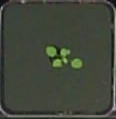
\includegraphics[width=.4\linewidth]{arabidopsis}
      \caption{Arabidopsis image from MMI database}
      \label{fig:sub1}
    \end{subfigure}%
    \begin{subfigure}{.5\textwidth}
      \centering
      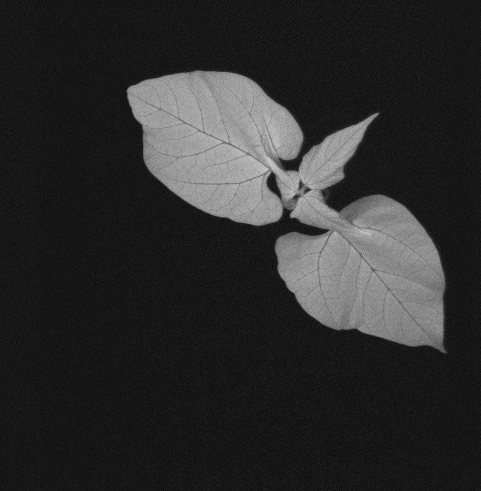
\includegraphics[width=.4\linewidth]{bean}
      \caption{Bean image from MMI database}
      \label{fig:sub2}
    \end{subfigure}
    \caption{Example of Multi-Modality Imagery Database images for training and validation}
    \label{fig:MMI}
\end{figure}

The total of the 751 images are divided into 2 sets with a split ratio of $60\%$ $40\%$, the training set with a total of 451 images and the validation set with a
total of 300 images. This can be performed by a script which randomly split the entire dataset into two or three sets and then recombine them into two or three files which
contains training, validation and optionally test set of images.

\subsection{Komatsuna Dataset}
Komatsuna, is a Japanese leaf vegetable, it belongs to the Brassica rapa family. This dataset consist of a 3d setup with two different kind of images. The 3D images are
divided into whole images containing the entire set of plants linked to a 3d image, these were collected on different days every four hours. These images, both RGB and
depth images, are $640\times 480$ in size, which will later be cropped according to what the network, in our solution, considers most appropriate. These images have been
placed at a distance of about 50cm from the plane, and have the following intrinsic matrix:

$$
\begin{pmatrix}
    382.641 & 0       & 223.248 \\     
    0       & 382.641 & 233.523 \\
    0       &       0 & 1
\end{pmatrix}
$$

We used these images as test images to validate the network trained specifically to recognize komatsuna leaves, and through the depth images and the intrinsic matrix
we sized the found leaves.

\begin{figure}[ht] 
  \centering
  \begin{subfigure}{.5\textwidth}
    \centering
    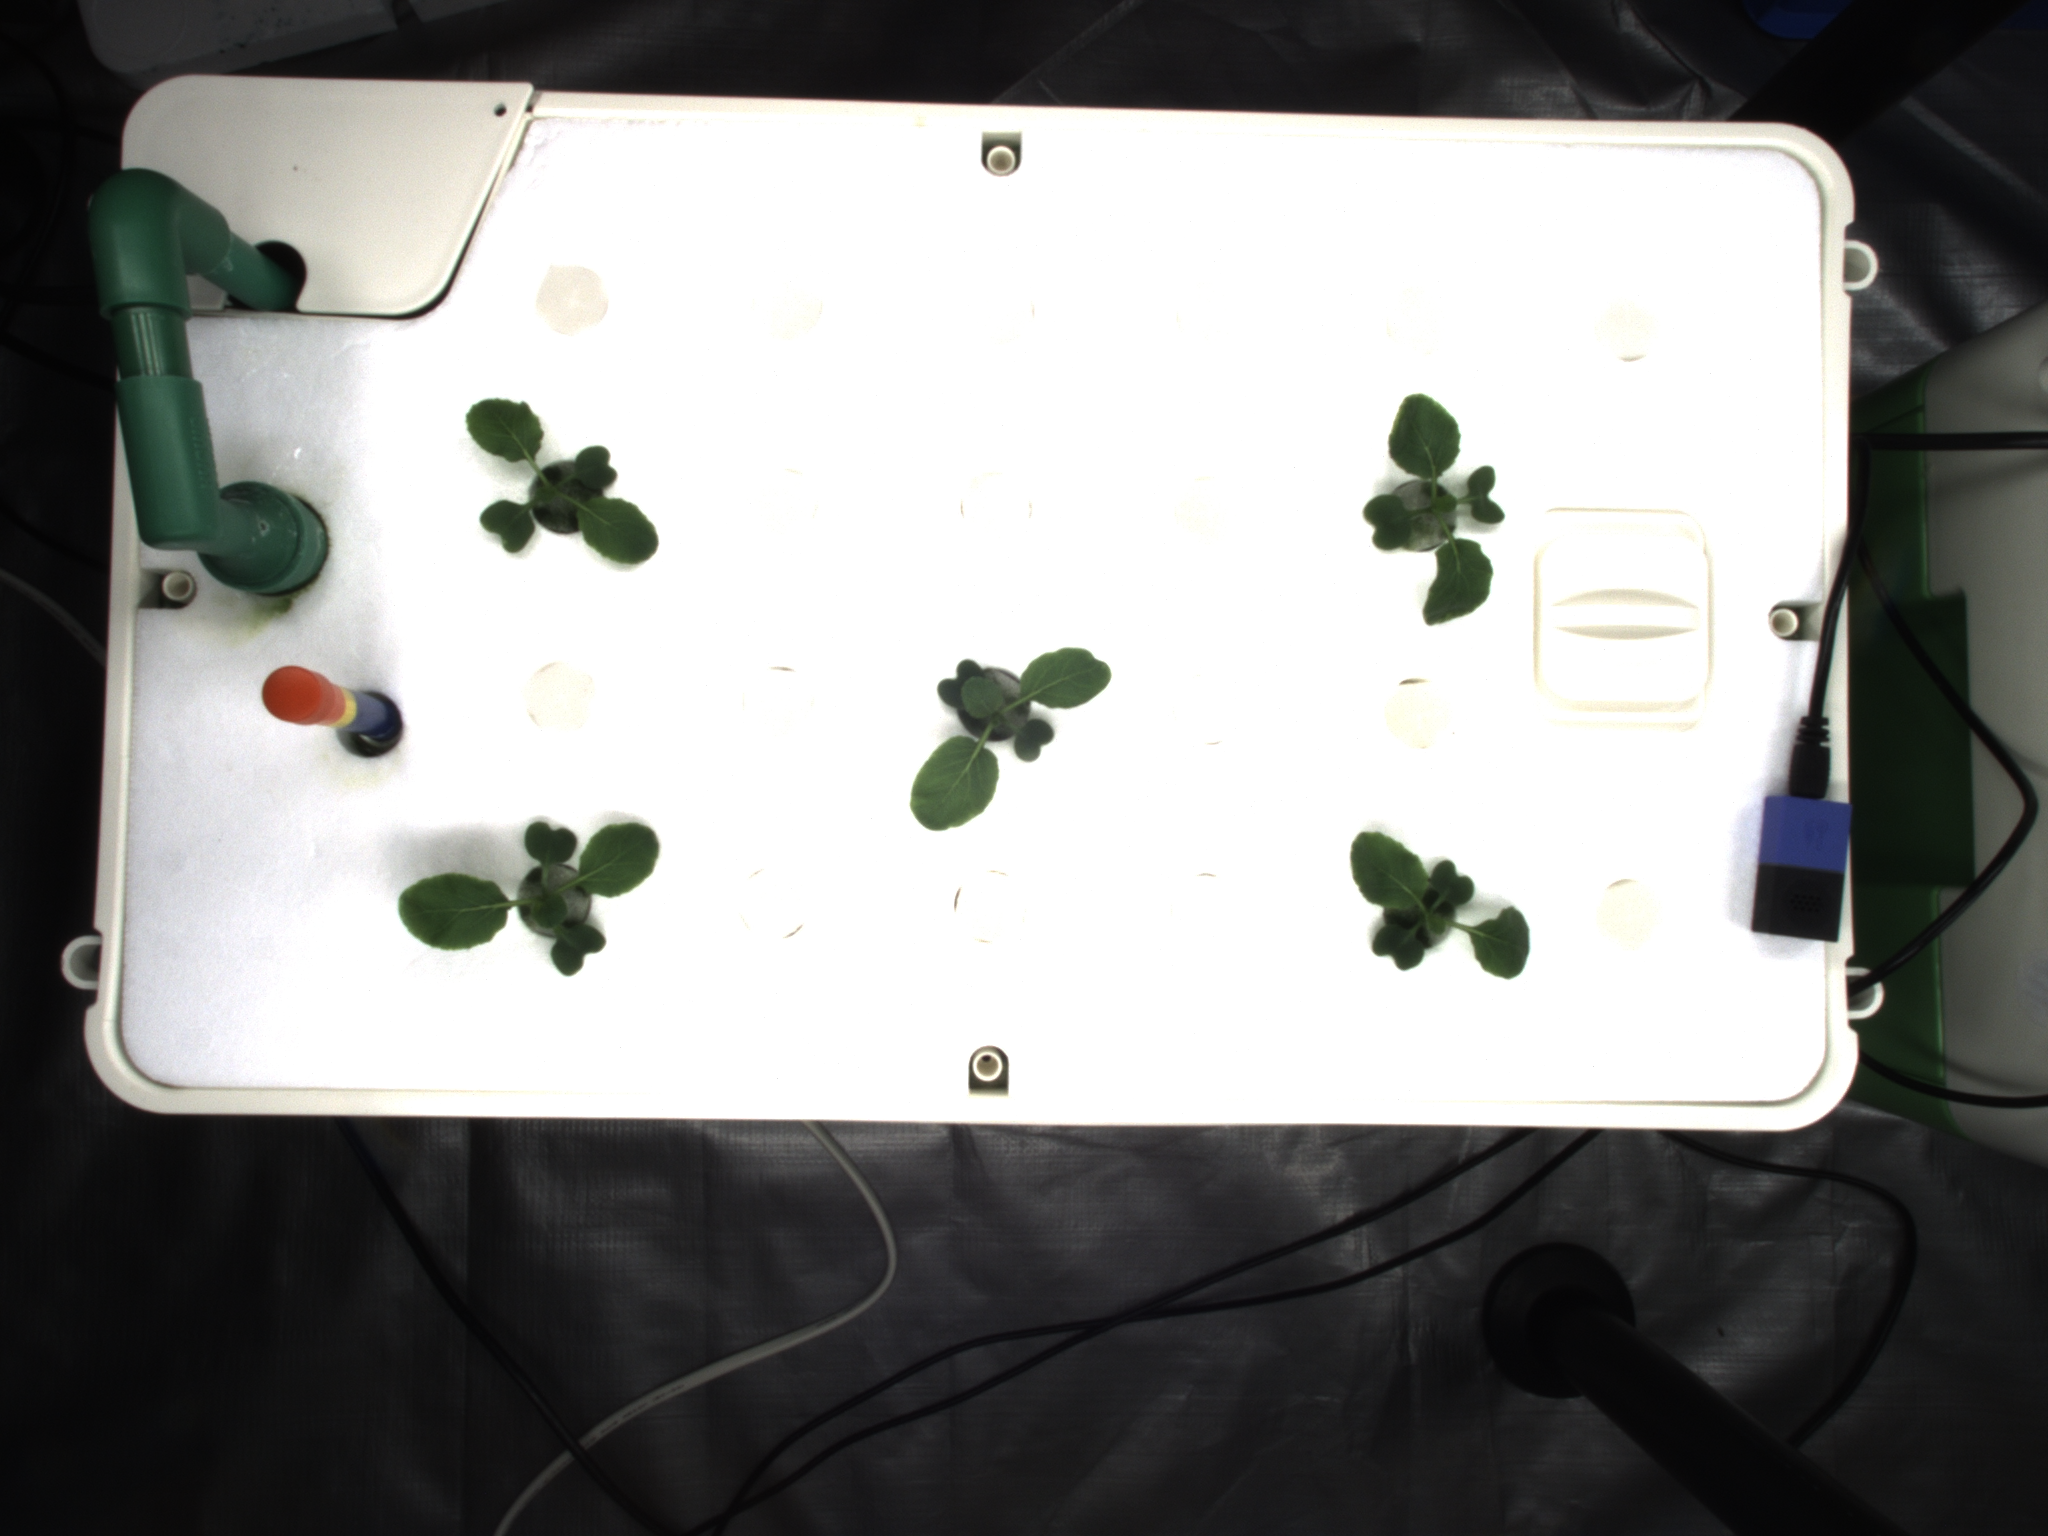
\includegraphics[width=.4\linewidth]{komatsuna_training}
    \caption{Training image for Komatsuna dataset}
    \label{fig:sub3}
  \end{subfigure}%
  \begin{subfigure}{.5\textwidth}
    \centering
    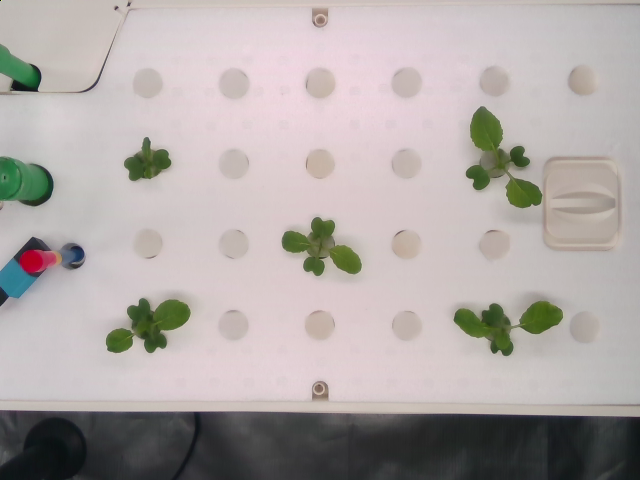
\includegraphics[width=.4\linewidth]{komatsuna_test}
    \caption{Test image for Komatsuna dataset}
    \label{fig:sub4}
  \end{subfigure}
  \caption{Komatsuna Dataset training, test images}
  \label{fig:komatsuna}
\end{figure}


The other images, concerning the multiview RGB, start from a higher dimension of $2048\times 1536$, without having the depth images. These have been divided plant by plant by
the authors obtaining a total of 900 images for the dataset with dimension $480\times480$. to improve even more the model obtained from the neural network we have increased
the dataset up to 4500 images, through the different techniques of rotation flip and blur, where we used 2700 images for training and 900 for validation, finally to test
the metrics we used the remaining 900 images.


\subsection{Our Dataset}
In our dataset we collect the most of images in a single day at a local farm, consisting of a set of images of basil seedlings. Some plants were subsequently collected
from which a second set of images was extrapolated over the next five days. The first set designed for training has a total of 128 images of size $640\times 480$
containing a total of 892 seedlings. All of these images have appropriately aligned depth images attached to them, so that 3D networks can also be trained. The second
set designed for testing consists of a set of images divided by days for a total of five days with 20 daily images. Their size is $1280\times 720$ with the depth images also
aligned. Each image consists of four seedlings rotated and swapped positions at each acquisition. On the last day, the dimensional information of the leaves that are
fully visible not covered by other leaves was also included.

\begin{figure}[ht] 
  \centering
  \begin{subfigure}{.5\textwidth}
    \centering
    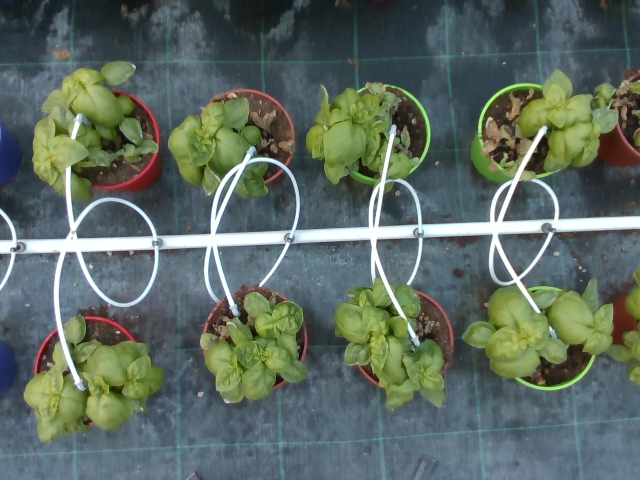
\includegraphics[width=.4\linewidth]{our_train}
    \caption{training image for our dataset}
    \label{fig:sub5}
  \end{subfigure}%
  \begin{subfigure}{.5\textwidth}
    \centering
    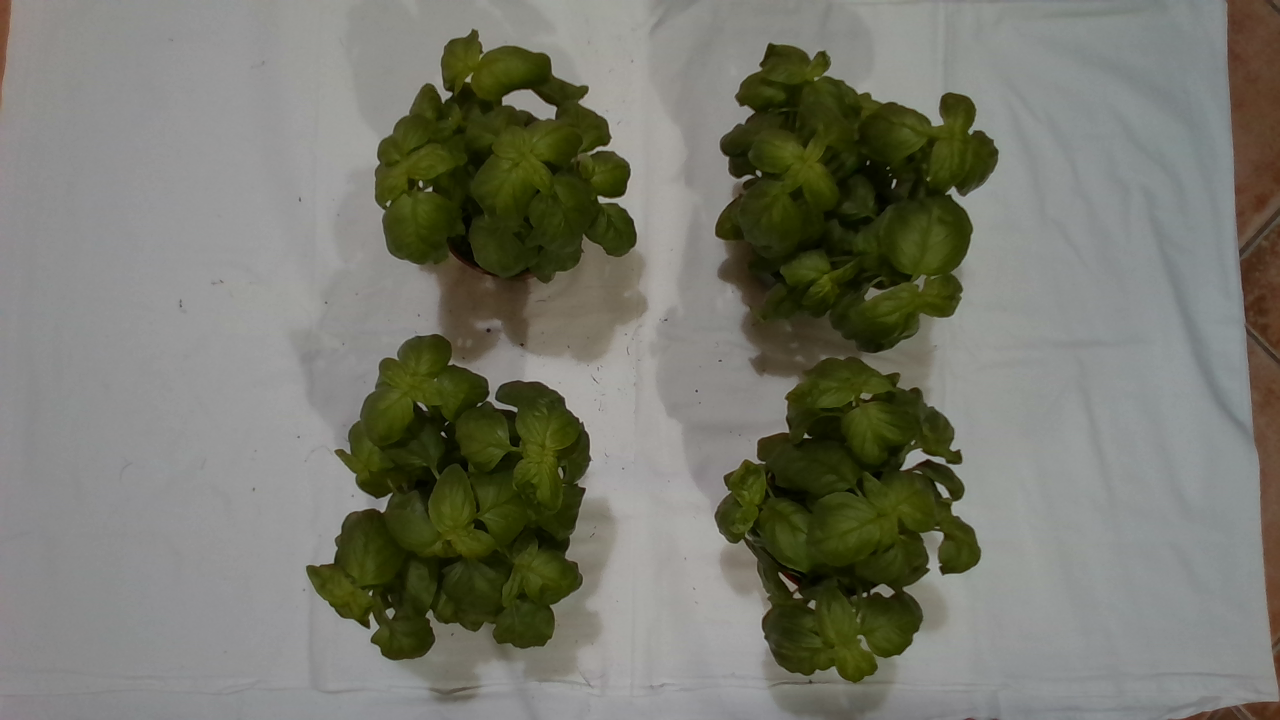
\includegraphics[width=.4\linewidth]{our_test}
    \caption{Test image for our dataset}
    \label{fig:sub6}
  \end{subfigure}
  \caption{Our Dataset training, test images}
  \label{fig:ourData}
\end{figure}

To be able then to do the dimensional calculation we made use of the intrinsic matrix provided by the camera used, an Intel RealSense D435:

$$
\begin{pmatrix}
    637.735 & 0       & 645.414 \\     
    0       & 637.735 & 349.205 \\
    0       &       0 & 1
\end{pmatrix}
$$

All images were acquired at a ground clearance of 92cm under varying but high light conditions. Placing a cloth in the background allowed us to adapt the network
trained via yolo for object detection to our dataset as well in order to automate the calculation of measurement validation.


\section{State of The art Comparison}



